\documentclass[10pt,a4paper]{article}
\usepackage[utf8]{inputenc}

% Define the page margin
\usepackage[margin=3cm]{geometry}

% Better typography (font rendering)
\usepackage{microtype}

% Math environments and macros
\usepackage{amsmath}
\usepackage{amsfonts}
\usepackage{amssymb}
\usepackage{amsthm}

% Define \includegraphics to include graphics
\usepackage{graphicx}

% Draw graphics from a text description
\usepackage{tikz}

% Syntax highlighting
\usepackage{minted}

% Set global minted options
\setminted{linenos, autogobble, frame=lines, framesep=2mm}

\title{Virtual Physics, Sheet 2}
\author{Marten Lienen (03670270)}

\begin{document}

\maketitle

\section*{Exercise 1}

\begin{minted}{modelica}
  model Pendulum

    parameter Real M_s = 250 "Mass of slider";
    parameter Real M_p = 70 "Mass of pendulum";
    parameter Real R = 2.5 "Radius";
    parameter Real I = M_p * R^2 "Angular inertial mass";
    parameter Real G = 9.81 "Gravitational acceleration";

    Real a_s;
    Real a_p;
    Real v;
    Real s;
    Real f_s;
    Real f_n;
    Real f_z;
    Real f_p;
    Real alpha;
    Real omega;
    Real phi;
    Real tau;

  initial equation

    v = 0;
    phi = 1.25;

  equation

    a_s = der(v);
    v = der(s);
    f_s = M_s * a_s;
    alpha = der(omega);
    omega = der(phi);
    tau = I * alpha;
    tau = f_n * R;
    f_n = M_p * (sin(phi) * G - cos(phi) * a_p);
    f_z = M_p * omega^2 / R;
    f_p + sin(phi) * f_z - cos(phi) * f_n - M_p * a_p = 0;
    a_p = a_s;
    f_p + f_s = 0;

    annotation (uses(Modelica(version="3.2.1")));
  end Pendulum;
\end{minted}

\section*{Exercise 2}

\begin{align*}
  \frac{d s}{d t} = v
\end{align*}
\begin{align*}
  \frac{d \phi}{d t} = \omega
\end{align*}
\begin{align*}
  \frac{d v}{d t} & = a_{s} = \frac{f_{s}}{M_{s}} = -\frac{f_{p}}{M_{s}} = \frac{f_{z}\sin(\phi) - f_{n} \cos(\phi) - M_{p}a_{p}}{M_{s}}\\
                  & = \frac{\left( \frac{M_{p}\omega^{2}}{R} \right)\sin(\phi) - M_{p} (G\sin(\phi) - a_{p} \cos(\phi)) \cos(\phi) - M_{p}a_{p}}{M_{s}}\\
                  & = \frac{M_{p}}{M_{s}} \left( \frac{\omega^{2}}{R} \sin(\phi) - G\sin(\phi)\cos(\phi) - a_{p} \cos(\phi)^{2} - a_{p}\right)\\
                  & = \frac{M_{p}}{M_{s}} \left( \frac{\omega^{2}}{R} \sin(\phi) - G\sin(\phi)\cos(\phi) - a_{p} (\cos(\phi)^{2} + 1)\right)\\
                  & = \frac{M_{p}}{M_{s}} \left( \frac{\omega^{2}}{R} \sin(\phi) - G\sin(\phi)\cos(\phi)\right) - a_{s} (\cos(\phi)^{2} + 1) \frac{M_{p}}{M_{s}}\\
                  & = \frac{\frac{M_{p}}{M_{s}} \left( \frac{\omega^{2}}{R} \sin(\phi) - G\sin(\phi)\cos(\phi)\right)}{1 + (\cos(\phi)^{2} + 1) \frac{M_{p}}{M_{s}}}
\end{align*}
\begin{align*}
  \frac{d \omega}{d t} = \alpha = \frac{\tau}{I} = \frac{f_{n}R}{I} = \frac{M_{p}(G \sin(\phi) - a_{p} \cos(\phi))R}{M_{p}R^{2}} = \frac{G \sin(\phi) - \frac{d v}{d t} \cos(\phi)}{R}
\end{align*}

\begin{minted}{python}
  #!/usr/bin/env python3

  from math import sin, cos

  # Parameters
  M_s = 250.0
  M_p = 70.0
  R = 2.5
  I = M_p * R**2
  G = 9.81

  # Initial conditions
  s = 0.0
  v = 0.0
  phi = 1.25
  omega = 0.0

  # Time step
  h = 0.001
  time = 0.0

  while time < 5:
      ds_dt = v
      dphi_dt = omega
      dv_dt = (M_p / M_s * (omega**2 / R * sin(phi) - G * sin(phi) * cos(phi))) / (1 + ((cos(phi))**2 + 1) * M_p / M_s)
      domega_dt = (G * sin(phi) - dv_dt * cos(phi)) / R

      s += h * ds_dt
      phi += h * dphi_dt
      v += h * dv_dt
      omega += h * domega_dt

      time += h
      print("{}\t{}\t{}".format(time, v, omega))
\end{minted}

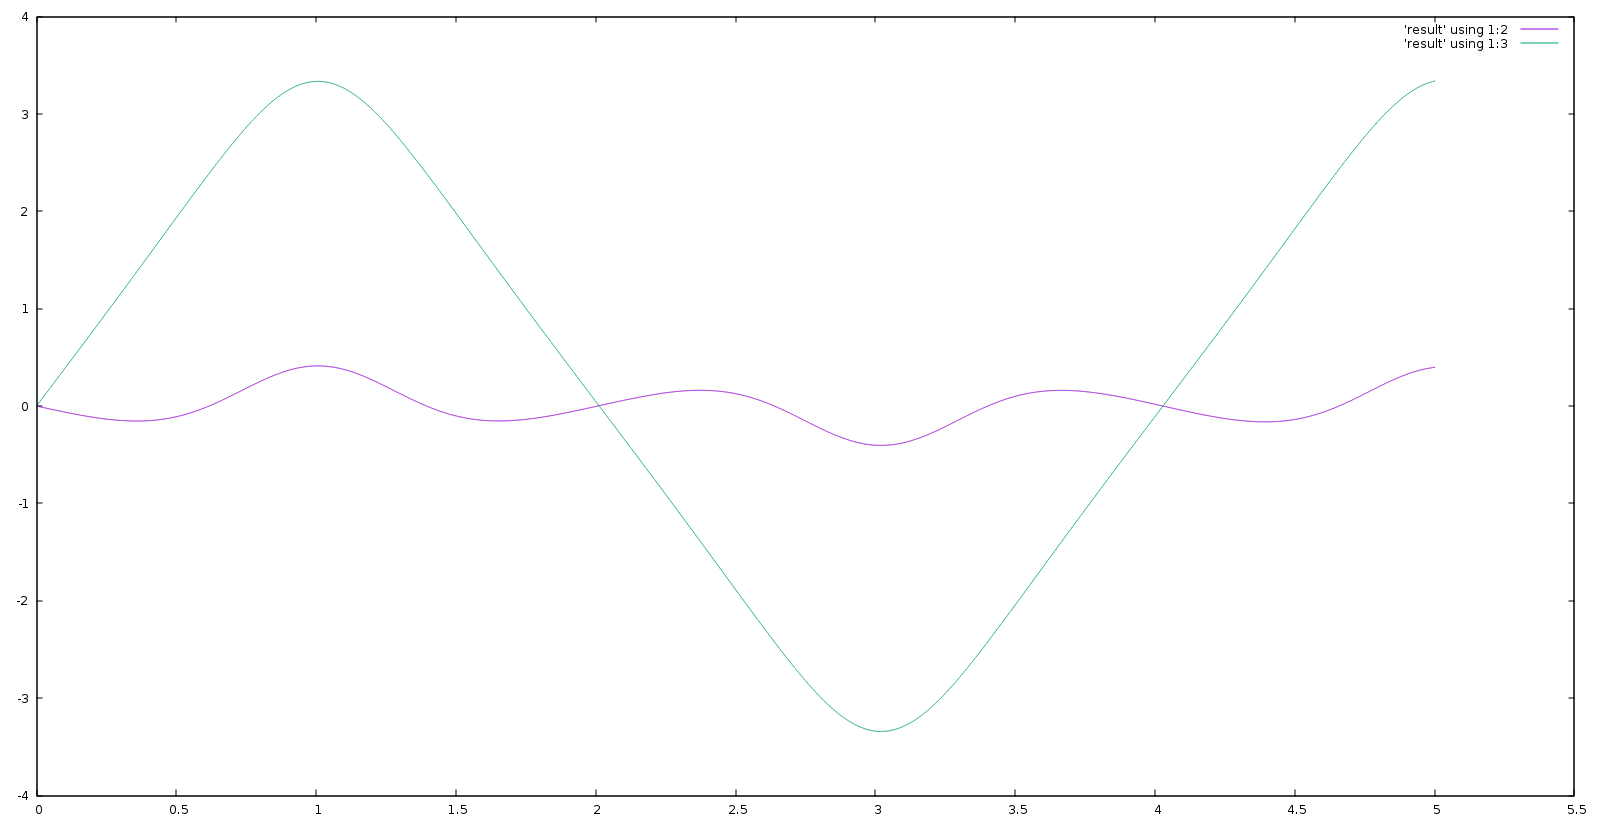
\includegraphics[width=450pt]{sheet-2/plot}

The graph looks almost exactly like the one I got in Dymola.
Also the graph of $\omega$ is inverted.
There is probably a sign error in one of the equations (or the lecturer made a sign error himself when he created the plot).

\end{document}
